\documentclass[
	ngerman,
	ruledheaders=section,%Ebene bis zu der die Überschriften mit Linien abgetrennt werden, vgl. DEMO-TUDaPub
	class=report,% Basisdokumentenklasse. Wählt die Korrespondierende KOMA-Script Klasse
	thesis={type=master},% Dokumententyp Thesis, für Dissertationen siehe die Demo-Datei DEMO-TUDaPhd
	accentcolor=9c,% Auswahl der Akzentfarbe
	custommargins=true,% Ränder werden mithilfe von typearea automatisch berechnet
	marginpar=false,% Kopfzeile und Fußzeile erstrecken sich nicht über die Randnotizspalte
	%BCOR=5mm,%Bindekorrektur, falls notwendig
	parskip=half-,%Absatzkennzeichnung durch Abstand vgl. KOMA-Script
	fontsize=11pt,%Basisschriftgröße laut Corporate Design ist mit 9pt häufig zu klein
%	logofile=example-image, %Falls die Logo Dateien nicht vorliegen
]{tudapub}


% Der folgende Block ist nur bei pdfTeX auf Versionen vor April 2018 notwendig
\usepackage{iftex}
\ifPDFTeX
	\usepackage[utf8]{inputenc}%kompatibilität mit TeX Versionen vor April 2018
\fi

%%%%%%%%%%%%%%%%%%%
%Sprachanpassung & Verbesserte Trennregeln
%%%%%%%%%%%%%%%%%%%
\usepackage[english, main=ngerman]{babel}
\usepackage[autostyle]{csquotes}% Anführungszeichen vereinfacht

% Falls mit pdflatex kompiliert wird, wird microtype automatisch geladen, in diesem Fall muss diese Zeile entfernt werden, und falls weiter Optionen hinzugefügt werden sollen, muss dies über
% \PassOptionsToPackage{Optionen}{microtype}
% vor \documentclass hinzugefügt werden.
\usepackage{microtype}

%%%%%%%%%%%%%%%%%%%
%Literaturverzeichnis
%%%%%%%%%%%%%%%%%%%
\usepackage{biblatex}   % Literaturverzeichnis
\bibliography{DEMO-TUDaBibliography}


%%%%%%%%%%%%%%%%%%%
%Paketvorschläge Tabellen
%%%%%%%%%%%%%%%%%%%
%\usepackage{array}     % Basispaket für Tabellenkonfiguration, wird von den folgenden automatisch geladen
\usepackage{tabularx}   % Tabellen, die sich automatisch der Breite anpassen
%\usepackage{longtable} % Mehrseitige Tabellen
%\usepackage{xltabular} % Mehrseitige Tabellen mit anpassbarer Breite
\usepackage{booktabs}   % Verbesserte Möglichkeiten für Tabellenlayout über horizontale Linien

%%%%%%%%%%%%%%%%%%%
%Paketvorschläge Mathematik
%%%%%%%%%%%%%%%%%%%
%\usepackage{mathtools} % erweiterte Fassung von amsmath
%\usepackage{amssymb}   % erweiterter Zeichensatz
%\usepackage{siunitx}   % Einheiten

\usepackage{graphicx}
\graphicspath{ {../images/} }

%Formatierungen für Beispiele in diesem Dokument. Im Allgemeinen nicht notwendig!
\let\file\texttt
\let\code\texttt
\let\tbs\textbackslash
\let\pck\textsf
\let\cls\textsf

\usepackage{pifont}% Zapf-Dingbats Symbole
\newcommand*{\FeatureTrue}{\ding{52}}
\newcommand*{\FeatureFalse}{\ding{56}}

\begin{document}

\Metadata{
	title=TUDaThesis - Abschlussarbeiten im CD der TU Darmstadt,
	author=Linnea Widmayer
}

\title{TUDaThesis -- Abschlussarbeiten im CD der TU Darmstadt}
\subtitle{Subtitle}
\author[L. Widmayer]{Linnea Widmayer}%optionales Argument ist die Signatur,
%\birthplace{Geburtsort}%Geburtsort, bei Dissertationen zwingend notwendig
\reviewer{Nico Faul \and Prof. Thomas Burg}%Gutachter

%Diese Felder werden untereinander auf der Titelseite platziert.
%\department ist eine notwendige Angabe, siehe auch dem Abschnitt `Abweichung von den Vorgaben für die Titelseite'
\department{etit} % Das Kürzel wird automatisch ersetzt und als Studienfach gewählt, siehe Liste der Kürzel im Dokument.
\institute{Institut}
\group{Arbeitsgruppe}

\submissiondate{\today}
\examdate{\today}

% Hinweis zur Lizenz:
% TUDa-CI verwendet momentan die Lizenz CC BY-NC-ND 2.0 DE als Voreinstellung.
% Die TU Darmstadt hat jedoch die Empfehlung von dieser auf die liberalere
% CC BY 4.0 geändert. Diese erlaubt eine Verwendung bearbeiteter Versionen und
% die kommerzielle Nutzung.
% TUDa-CI wird im nächsten größeren Release ebenfalls diese Anpassung vornehmen.
% Aus diesem Grund wird empfohlen die Lizenz manuell auszuwählen.
%\tuprints{urn=XXXXX,printid=XXXX,year=2022,license=cc-by-4.0}
% To see further information on the license option in English, remove the license= key and pay attention to the warning & help message.

% \dedication{Für alle, die \TeX{} nutzen.}

\maketitle

\affidavit% oder \affidavit[digital] falls eine rein digitale Abgabe vorgesehen ist.
% Es gibt mit Version 3.20 die Möglichkeit ein Bild als Signatur einzubinden.
% TUDa-CI kann nicht garantieren, dass dies zulässig ist oder eine eigenhändige Unterschrift ersetzt.
% Dies ist durch Studierende vor der Verwendung abzuklären.
% Die Verwendung funktioniert so:
%\affidavit[signature-image={\includegraphics[width=\width,height=1cm]{example-image}}, <hier können andere Optionen wie z.B. affidavit=digital zusätzlich stehen>]

\tableofcontents

\chapter{Einleitung}

\chapter{Methode}
\chapter{Ergebnisse}
	% !TeX spellcheck = en_US


\section{Lipids}

In the previous chapter, the method of using a sacrificial layer to detach Ice was discussed. For this, lipids need to be solved at cryogenic temperatures. As not every lipid is solvable the same way in different solvents, a first test is conducted to obtain the potential solvents at room temperature. then the best solvents are also tested at cryogenic temperatures.

The solubility of lipids at room temperature in different solvents are tested. For this experiment the cover glasses are coated with lipids. Then a first reference image was taken. Then the cover glass is given into a small container with the potential solvent. After 15 minutes, the cover glass is removed and compared under the microscope with the reference picture. If streaks created from lipids are still as visible as before, the lipids are categorized as insoluble in this solvent. If the streaks partially dissapeared and/or are less visible, the lipids are categorized as partially soluble in this solvent. Last if the streaks completely disappear, the lipids are assinged as soluble in the solvent (Table \ref{table:LoeslichkeitRaumtemperatur}).


\begin{table}[hbt!]
	\centering
	\begin{tabular}{|l|c|c|}
		\hline
		potential solvent & solubility EGG-PC & solubility DOPC \\
		\hline
		\hline
		4-Methyl Pentene & soluble & N/A  \\ 
		\hline
		3-Methyl Pentene & slightly soluble & insoluble \\
		\hline
		1-Pentene & insoluble & insoluble \\
		\hline
		Isopentane & soluble & slightly soluble\\
		\hline
		1-Propanol & soluble & soluble\\
		\hline
		Pentane & soluble & insoluble\\
		\hline
		Ethanol & N/A & soluble\\
		\hline
	\end{tabular}
	\caption{result of solubility tests at room temperature. soluble indicates solvents which are able to visibly solve all lipids off a cover glass. slightly soluble indicates solutions which are able to solve lipids, but some stains are left: insoluble indicates no visible changes of tested lipid.}
	\label{table:LoeslichkeitRaumtemperatur}
\end{table}

This experiment shows that three different solvent exist for each EGG-PC as well as DOPC with high solubility (Table \ref{table:LoeslichkeitRaumtemperatur}). Following those results, solvents categorized with "soluble" are tested regarding solubility at temperatures of \SI{-140}{\degreeCelsius}. As not all solutions are liquid at \SI{-140}{\degreeCelsius} (Table \ref{table:SchmelztemperaturLösungsmittel}), they are tested at higher temperatures above their melting point, as mentioned in chapter \ref{chapter:meltingtemp}. In addition they are tested as mixtures with other solvents with a lower melting point, to lower its melting point. Additionally all lipids are tested in liquid ethane. Ethane was not tested at room temperature, as the boiling point is at \SI{-88.6}{\degreeCelsius} (ZITAT PUBCHEM ETHANE).

This experiment shows that no tested solvent was able to completely solve lipids at \SI{-140}{\degreeCelsius} and within \SI{15}{\minute} (Table \ref{table:Cryoloeslichkeit}). Also the smears of lipids did not only stay partially behind, but also new streaks appear on the glass slides. This means that some lipids redistributed on the glass slide.

Using solvents to destroy a sacrificial layer, a high solubility is a requirement. In this case, the sacrificial layer would be completely covered by the ice layer except the edges. So the solvents have only a small area to start solving the layer. To solve it completely, a strong solvent is needed to detach the ice layer from the slide. Additionally, as the ice layer needs to stay vitrified, the temperature cannot be raised over \SI{-140}{\degreeCelsius}. 

The solving process of lipids in solutions is probably endothermic. This means that heat is needed to solve lipids, so cold temperature heavily decrease solubility QUELLE DENNIS ODER SO. This effect was observed over the last experiments by all solvents to varying degree. It can be assumed that the majority of solvent lipids mixtures are endothermic which is very disadvantageous for finding a potential solvent lipid candidate. Strongly exothermic solvents could heat up the ice enough to create ice crystals, which would not be feasible. So only weakly exothermic solvents are feasible for this task. 

\begin{table}[hbt!]
	\begin{subtable}{\linewidth}
		\centering
		\begin{tabular}{|l|l|}
		\hline
		Solvent & Result \\
		\hline
		\hline
		Pentane & soluble at \SI{-125}{\degreeCelsius} \\
		\hline
		4-methyl pentene & insoluble \\
		\hline
		\makecell[l]{1:1 volume ratio\\ HFE to 1-Propanol} & \makecell[l]{did not mix,\\ slightly soluble}\\
		\hline
		Liquid ethane & insoluble\\
		\hline
		\end{tabular}
		\caption{EGG-PC}
		\label{table:EGG-PCCryoloeslichkeit}
	\end{subtable}
	\begin{subtable}{\linewidth}
		\centering
		\begin{tabular}{|l|l|}
		\hline
		Solvent & Result \\
		\hline
		\hline
		\makecell[l]{1:4 volume ratio\\ 1:2 molar ratio\\ Ethanol to Isopentane} & slightly soluble\\
		\hline
		\makecell[l]{1:2 volume ratio\\ 1:1 molar ratio\\ 1-Propanol to Isopentane} & insoluble \\
		\hline
		Isopentane & slightly soluble\\
		\hline
		1-Propanol & \makecell[l]{at \SI{-130}{\degreeCelsius}\\ slightly soluble}\\
		\hline
		Liquid ethane & insoluble \\
		\hline
		\end{tabular}
		\caption{DOPC}
		\label{table:DOPCCryoloeslichkeit}
	\end{subtable}
	\caption{ in \ref{table:EGG-PCCryoloeslichkeit} for EGG-PC, no sufficient solubility at -140°C was found. In \ref{table:EGG-PCCryoloeslichkeit}, DOPC was tested but also no proper solution was found.}
	\label{table:Cryoloeslichkeit}
\end{table}

As finding a good solvent lipid combinations seems very unlikely, a new method was tested. In the next section, the finger tool is used to try mechanically detach the ice layer.

\FloatBarrier
\section{Finger}

For this section, cover glass coated in Parylene are used as object slide. The slide is then dipped in solution containing lipids for a lipid coating. A ice layer with fluoriscine is frozen with either plunge-freezing or using a pincer and liquid nitrogen. Additionally, the "finger" is used as tool to try lifting off a piece of ice from the frozen layer on top of the lipids. In the next sections, different variables are examined and tested.

\subsection{Finding right dosage of HFE}

First obvious variable and potential issue source is the amount of HFE used as glue. High dosages of liquid hfe can spread underneath the frame holding the sample, leading to an inefficient force distribution. Also a big glue layer is a weak point between finger and sample, leading to a reduction of maximum force which can be applied. Too little glue will not connect the finger to the sample. Additionally, the dosaging of glue revealed to be a big challenge.

The HFE is dosaged with a pipette. The HFE is "taken up WORD" at room temperature, then the HFE is "released WORD" on the tip of the finger. In between, HFE is evaporating. Around $4\,\mu l$ is evaporating each time. Based on this knowledge, dosaging $4.10\,\mu l$, $4.30\,\mu l$ and $4.50\,\mu l$ is compared and a picture is made.

Results show that pipetting HFE is not reliable. The range spreads of too little to too much HFE even for those dosages. Not only differences in evaporation are playing a role. Correct placement on the tip is a major factor of glue dosaging. Still, a visual estimate for the correct glue dosage can be made by calculating the drop volume out of camera images.

\begin{figure}[hbt!]
	\centering
	\begin{subfigure}[]{0.45\textwidth}
		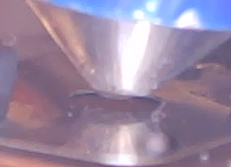
\includegraphics[width=6cm]{Temp_Picture_Lower_Limit}
		\caption{chosen example for lower limit}
	\end{subfigure}
	\begin{subfigure}[]{0.45\textwidth}
		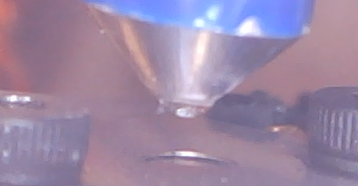
\includegraphics[width=6cm]{Temp_Picture_Upper_Limit}
		\caption{chosen example upper limit}
	\end{subfigure}
	\caption{example of upper limit and lower limit for glue dosages. (BETTER PICTURES NEEDED)}
\end{figure}

To calculate the actual glue dosage, two exemplary Pictures of an Upper and lower limit of glue dosages is picked. Then the Volume is calculated with a formula for the volume of a spherical section. All needed components are calculated out of the estimated contact angle of the glue $\alpha \approx 45°$ and the tip diameter of $d = 1.68\,mm$, for the lower range a reduction of $d$ by a factor of $\frac{2}{3}$ is assumed as the drop is not covering the whole tip. The resulting volume range of the glue dosage is $ 0.11\,\mu l \gtrapprox V \gtrapprox 0.38\,\mu l $. Also the lower end of this range is desired, but the repetition range in correctly dosaging lower doses is lower.

\subsection{Temperature over applied force}

As the HFE gluing effect is temperature dependent, the temperature needs to be regulated precisely. To narrow in the temperature dependency of HFE, the properties of HFE are observed at different temperatures in a regulated bath. Between -160°C and -170°C, the HFE is increasingly viscious. Under this temperature, HFE Freezes and gets brittle. Over this temperature range, HFE is too fluid to transfer any tensile forces. 

In application tests on lipid samples, the temperatures -160°C, -165°C and -170°C are compared. It was observed that decreasing temperatures lead to higher forces transferred to the sample. At the same time, temperatures are not reliably reached under -160°C.
As lower temperatures leads to an additional factor for repeatability issues, -160°C is used all other experiments.

\subsection{Tensile mode vs Shear mode}



\subsection{Detaching ice with finger of plunge freezed samples}

Next observed possible factor is the thickness of the ice layer. In the following, samples freezed with a plunge-freezer are compared to samples freezed with a pincer in liquid nitrogen. The results are categorized in 4 categories: Not successful pulls don't have visible changes of the flourescent ice layer, Partially successes are visible breaks or clear movement of ice parts on the ice layer, Successful liftoff is a missing piece and a visible piece on the finger, which could be used for future steps. In the results, there is no difference between Hand freezed and plunge-freezed samples regarding detachability. Therefore Ice thickness is not a factor which makes detaching ice easier. As both methods don't show success in detaching ice pieces, it could still be a relevant factor but not a thing which should make a certain solution magically work xD

\subsection{other observed error sources??}

Wrong positioning, forming of ice

\begin{table}
	\centering
	\begin{tabular}{|c|c|c|}
		\hline
		Category & Hand-freezed & Plunge-freezed \\
		\hline
		\hline
		count executed tries & 4 & 4\\
		\hline
		unsuccessful & 3 & 3\\
		\hline
		breaks/movement of ice & 1 & 1\\
		\hline
		piece lifted with finger & 0 & 0\\
		\hline		
	\end{tabular}
	\caption{Comparison of detachability between hand-freezed and plunge-freezed samples}
\end{table}

\section{PDMS}

Now two mixture ratios of PDMS are compared. For this, samples where coated with 4:1 and 1:2 curing agent to base coat weight ratio. Also for ..., glass without pdms is used. The pulling mashine was used to determine the max force. A plexiglass stamp was used for pulling off the PDMS layer. UV Glue was used to fixate the plexiglass onto the PDMS and is cured with 3 min UV exposure. After pulling, the Area of the separating layers is determined via microscope. Then the max pulling tension is calculated. This was repeated several times. The Result shows, that glass is hardest do pull off. Then 4:1 is harder to separate than 1:2 (Fig. \ref{fig:vgl4:1zu1:2zuGlas}). In literature, 1:2 weight ratio should have a lower adhesion force on ice too\cite{IbanezIbanez.2022}. For those reasons, 1:2 was picked to continue experiments with plasma treatment.

\begin{figure}
	\centering
	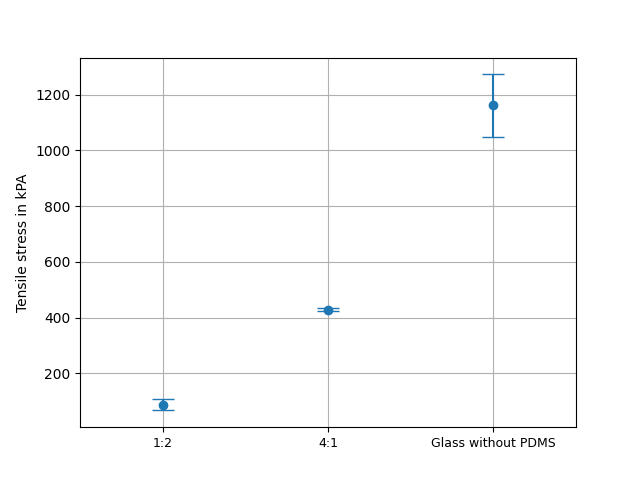
\includegraphics[width=14cm]{plotVGLZugspannungPDMSMischungsverhaeltnisse}
	\caption{Comparison 4:1, 1:2 Base coat to curing Agent and glass without PDMS}
	\label{fig:vgl4:1zu1:2zuGlas}
\end{figure}

\begin{figure}
	\centering
	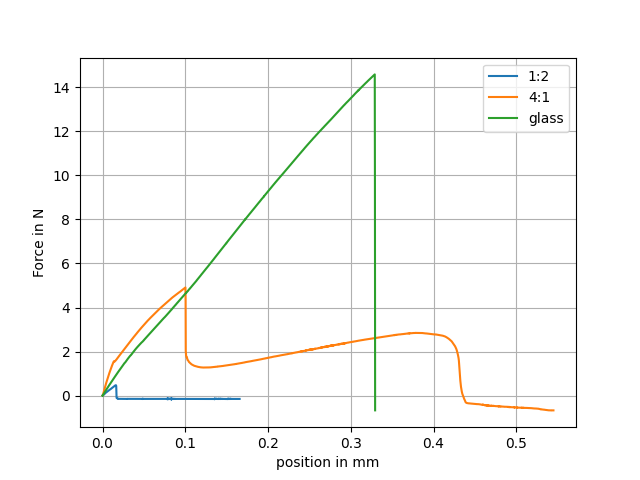
\includegraphics[width=14cm]{ForceOverTime}
	\caption{force over Time}
\end{figure}

In the next experiment, the effect of plasma curing is investigated. The same setup is used. Samples with a 2:1 weight ratio are additionally plasma treated before quickly clamping on the pulling mashine. Even with low repetition rates, a clear tendency can be observed. With lower and stronger plasma treatment, the durable the PDMS Layer gets (Fig. \ref{fig:PlotPlasmaAktivierung}). Over the whole range, The needed stress sextubles. Because the repititon rate is low, the exact values should be treated cautiosly. Also the results are not applicable to other mixture ratios, as different behaviour in plasma activation was observed between 2:1 and 4:1 weight ratio. also no glass-like state was observed in 2:1 weight ratio mixture.


\begin{figure}[h]
	\centering
	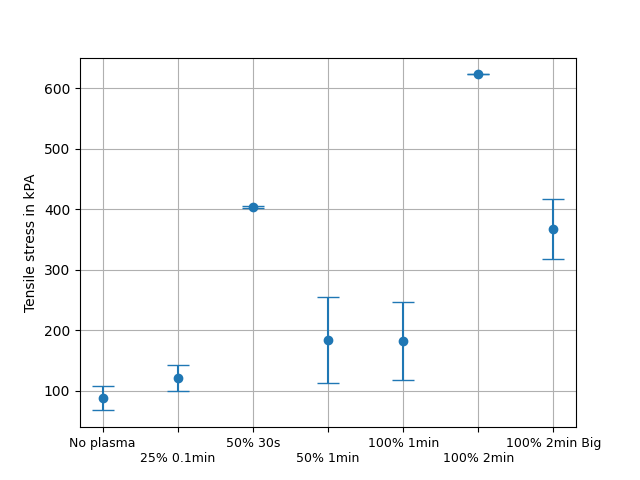
\includegraphics[width=14cm]{plot2_1PlasmaAktivierung}
	\caption{PDMS 2:1 Comparison between various Plasma curing strengths and durations.}
	\label{fig:PlotPlasmaAktivierung}
\end{figure}




\chapter{Diskussion}
\chapter{Zusammenfassung}
\chapter{Schluss}

\chapter{Quellen}
\printbibliography

\end{document}
